\subsection{Heterogeneous sensor systems}
\subsubsection{Heterogeneous capacitive arrays}

\begin{minipage}{\linewidth}
\centering
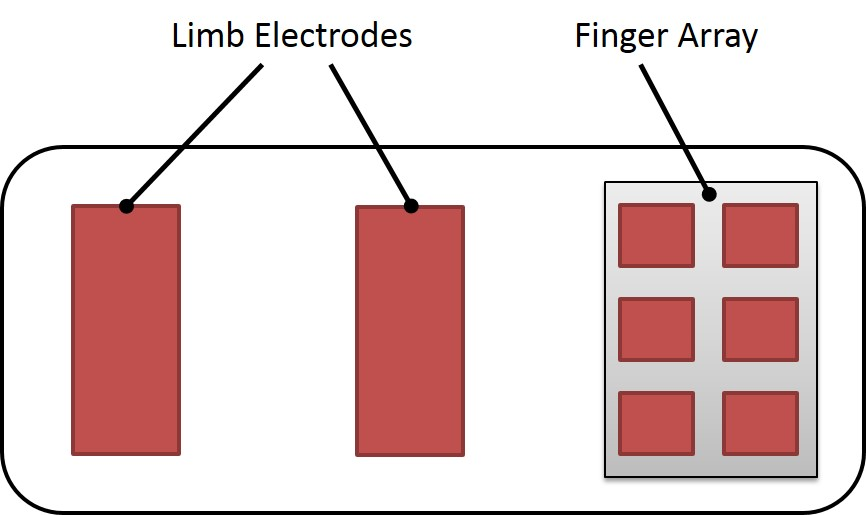
\includegraphics[width=0.4\textwidth]{images/proc_hetero_array}
\captionof{figure}{Heterogeneous sensor array for limb detection and finger tracking}
\label{fig:proc_hetero_array}
\end{minipage}

Figure 1 Active armrest sketch - six electrodes for finger gesture detection in front, two for arm detection in back
We briefly mentioned the challenge of using the armrest as an interactive zone. It is necessary to clearly distinguish between intended control gestures by the driver or if he is just resting the arm. Our approach is to use the status of both arm and hand to identify the intention. Capacitive proximity sensors create a weak electric field that is disturbed by conductive objects, e.g. limbs and fingers. They can be used to detect posture and realize free-air gesture interfaces. We are combining both methods to enable both intention recognition and small finger gestures.
3.1	Interaction concept

Figure 2 Postures of limbs on armrest - resting position (left),  arm raised position (middle), hand raised position (right).
In Figure 2 we can see the three different positions arm and hand can have on the armrest. On the left arm and hand are in resting position with both close to the surface. The middle image shows the arm raised position and fingers touching the front of the armrest. The right picture shows the arm resting on the back and the hand in proximity of the front area. The latter two positions are suitable for finger-based gestural interaction as they can be moved freely. The system should therefore be able to distinguish between the three different positions.
The interaction for both active positions is a bit different. Regarding the arm raised position the person will typically want to interact using familiar touch gestures. In the hand raised position it is necessary to track gestures that are performed in the air. In both cases we assume that a single finger is used. A set of four different gestures has been defined for both interaction methods. The number is sufficient to control the user interface that we have developed and support both navigation and selection. The type of gestures has been defined after looking at previous research into touch and hand gestures [3, 14]. For the touch interaction we support left and right swipes performed with either one or multiple fingers. Regarding the free-air interaction we are using left and right swipes, as well as circles either clockwise or counter-clockwise. The gestures are mapped to typical navigation and selection options required to trigger the different actions of the GUI that we will describe in the prototype section.
3.2	Data processing
 
Figure 3 Arm model and detection of posture based on distances to two sensors and finger array for resting position (1), hand raised position (2) and arm raised position (3)
The data processing of the Active Armrest requires three distinct steps. At first we have to determine the three potential limb postures specified in the previous section. Afterwards, we need to calculate the position of the fingers in or above the interaction area, and finally perform a time-series analysis of subsequent positions to infer different gestures. 
A stylized view of the posture detection is shown in Figure 4. The two distinct arm sensors are able to determine single distance values. In addition the aggregated data of the finger detection array in the front is used to detect a third distance value. To map the different postures we are using a set of thresholds that determine if the arm or hand is touching the armrest surface, or is hovering above it. As we are acquiring sensor data proportional to distance it is also possible to calculate orientation angles of the arm and use it as input. However, we are not using that option in this work.
The calculation of the finger position in three dimensions is adapted from the method presented by Braun et al [4] that uses a combination of weighted average for planar location and stepwise linear interpolation to determine the height. An addition is the distinction of one and multiple finger touch events, distinguished by an additional threshold.
To classify the gestures we are using points from a distinct start to a distinct stop. In case of the free-air interaction this is determined by the finger moving (exceeding a certain gradient between subsequent points) and stopping to move. In case of the touch interaction it is determined also by a finger starting and stopping to move, however only when in touch distance. The points between start and stop position are normalized to a specific time-scale and we are using five significant positions in this time frame that are fed into a SVM classifier. There are distinct classifiers for the two different methods that are triggered according to the selected interaction pattern. The SVM is trained using the sequential minimal optimization method by Platt [11].
	
%Figure 25 Data processing pipeline of Active Armrest
As we already mentioned, the Active Armrest electrodes are put into two groups. The data processing for both groups is distinctly different. In order to detect the presence of the arm using the two-electrode group a simple threshold on the accumulated values is used. The six sensor array in the front (touch area) is using the presented weighted average method to calculate finger positions. Additionally a threshold is used to distinguish one and two fingers. Overall there is a data processing pipeline as shown in Figure \ref{fig:armrest_proto}. The finger tracking and gesture recognition will be inactive until it is ensured that no arm is present. 

\subsubsection{Heterogeneous sensor fusion}
\begin{figure}[h]
\centering
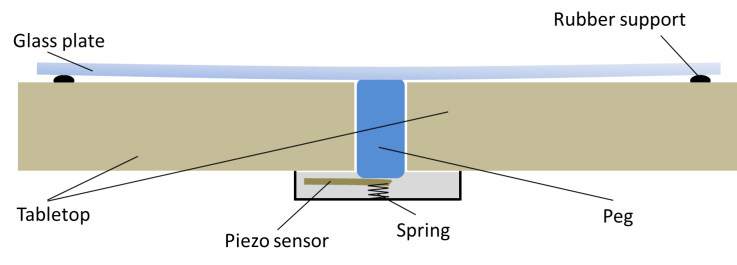
\includegraphics[width=0.7\textwidth]{images/captap_peg}
\caption{Suspended peg knock detection system for CapTap \cite{Braun2013ChairAid}}
\label{fig:captap_peg}
\end{figure}
%Figure 34 Suspended peg knock detection system for CapTap [80]
The hand location of the CapTap is similar to the methods presented for the MagicBox. We add the additional component of knock detection to provide selection events when touching the surface. Figure \ref{fig:captap_sketch} shows a sketch of the knock detection system. The table has a glass plate that is suspended on some rubber supports. In the center of the table we attach a small peg (enlarged in sketch) that creates a connection between the glass plate and a piezo sensor. If the glass plate starts vibrating from a touch we can measure this using the piezo sensor \cite{Braun2013ChairAid}. If a notable vibration is measured we are collecting the next 50 samples, resulting in a window of 250 milliseconds. To distinguish single and double knocks we calculate the weighted average within this window to get a measure for the distribution of sensor values within. If the average is closer to the beginning of the window the resulting event should be a single knock, and a double if the average is closer to the end of the window.
Hand localization and knock detection are working independently and are combined later in the software. It is reasonable to combine this, e.g. to ignore knock events that are occurring without a hand present. They may be indicative of a person doing a strong step close to the table.